\chapter{Exp2: Robot reaching}

To investigate whether the previous simulated experiment would generalize to
real robotic arms, robots were set up to perform a reaching task, where a
central server maintained a replay buffer, parameters, and executed training.
Data collection was distributed over three robots with respective computers.

\section{Method}

\subsection{Algorithms and Equipment}

The same NAF implementation as in the previous simulated experiment was used,
but with the modifications for distributed data collection. The same reward
function as in the first simulated experiment was used. For smoother
trajectories, the action output $\mu$ of the network was instead scaled by
$0.01$, making the arm move no more than $1$ cm per iteration. The policy was
trained on a separate server equipped with a GPU.  Three 3-DoF robotic arms
controlled by cartesian commands were used. For every arm, there was one
dedicated computer each that evaluated the latest policy given the arm pose and
sent the transitions to the server. The entire setup (excluding server) is
shown in the bottom part of figure \ref{fig:workspace_lidar_place}. In order to
facilitate communication of recorded state transitions and fetching updated
parameters, a server was implemented enabling PUT and GET requests from the
local workers.

\subsection{Data gathering}

Before and after each action was sent to the robot arm, poses of the arm were
measured. This process could only be done at approx. $2-4$ Hz, not including
arm re-positioning for environment reset, making re-runs from scratch time
consuming. Therefore, data gathering was first run on the three robots for $4$
hours without policy updates, resulting in approximately $80k$ state
transitions. The actions during the data collection-only phase were randomly
drawn from $\mathcal{N}(\mathbf{0}, 0.005^2 \mathbf{I})$, and when the robot
arm reached outside the workspace, or reached within $1$ cm of the target, the
end-effector was replaced at a new random starting position. The commands were
2-dimensional vectors representing the relative movement in $x$ and $y$
direction respectively. The $z$-coordinate was kept fixed during the
experiment. When training of the parameters was started on the server, the
robots kept collecting and pushing data to the server, and synchronized
parameters before each reset of the end-effector position. During this phase,
noise was added to the policy during every 3 out of 4 runs, while every 1 out 4
runs the policy was evaluated without noise in order to track progress.

\section{Results}

The performance of the policy was evaluated by measuring the average distance
to the target position on the last state before every reset. The progress of
this metric is shown in figure \ref{fig:uarm_moving_goal_progress}, here shown
with a running mean of width $128$. The trained policy and value function are
shown in figure \ref{fig:uarm_moving_goal_policy}. The distributed version of
NAF solves the task of approaching arbitrarily set goals on a set of
distributed real-world robots.

\begin{figure}[h!]
    \centering
    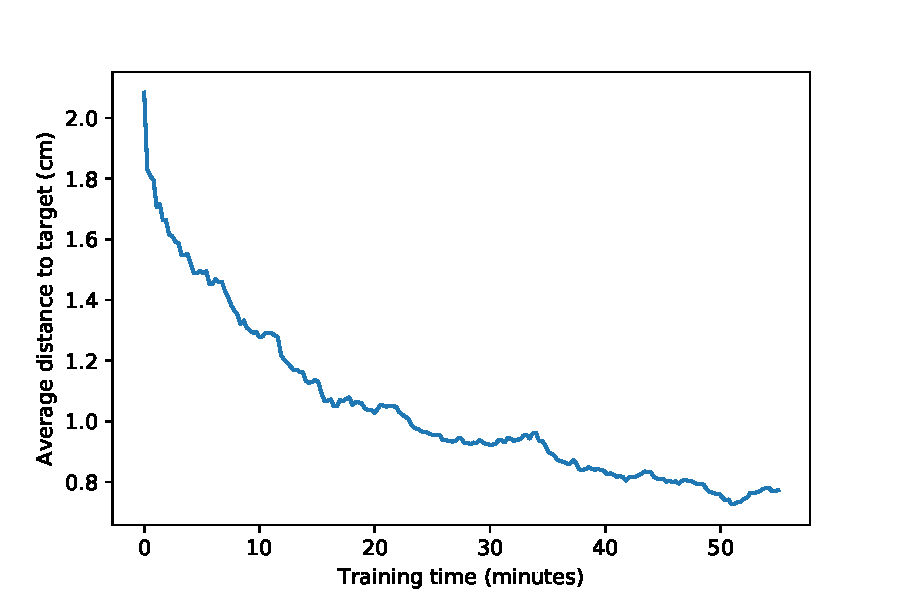
\includegraphics[width=0.50 \textwidth]{res/uarm_moving_goal_progress.pdf}

    \caption{Average final distance of end-effector to randomly set target
    poses learned using a pool of robots collecting experience. NAF was used
    for training the policy on a separate server from a growing set of
    transitions sent from the collecting robots.}
    \label{fig:uarm_moving_goal_progress}
    
\end{figure}

\begin{figure}[h]
    \centering
    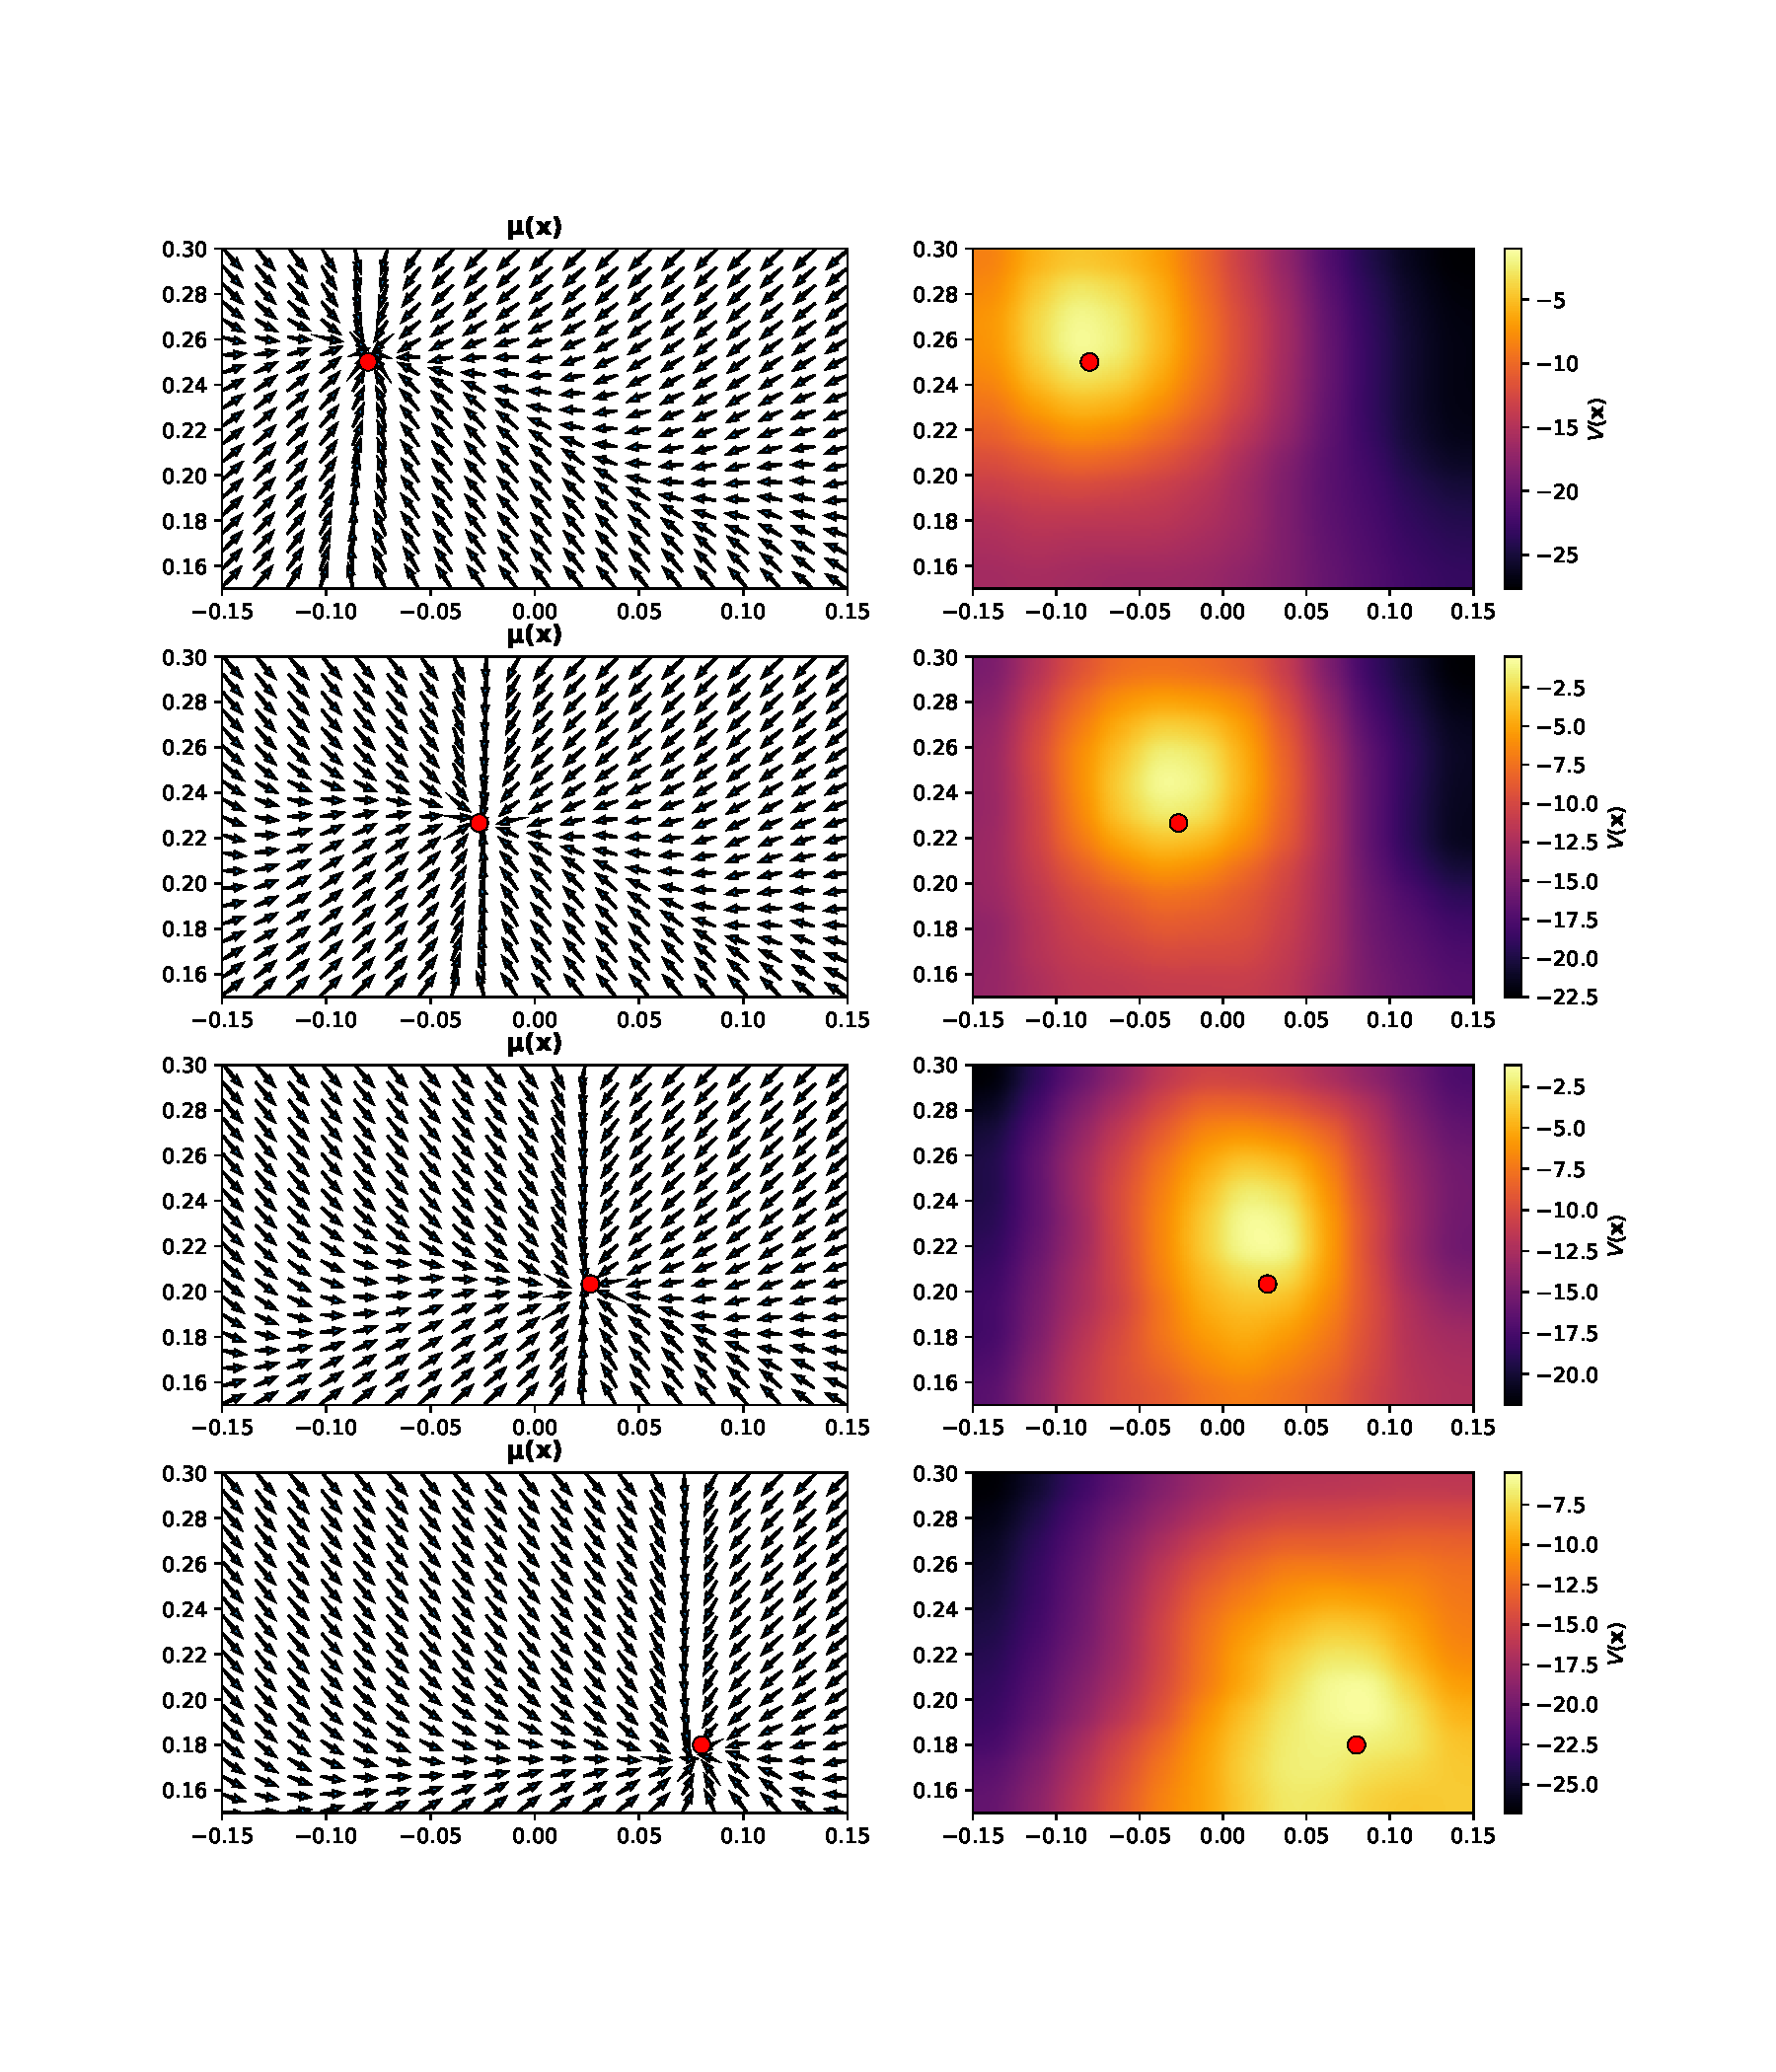
\includegraphics[width=\textwidth]{res/multiple_goals_uarm.pdf}

    \caption{Learned policy using NAF with distributed collection of experience
    from real-world robots.}

    \label{fig:uarm_moving_goal_policy}
    
\end{figure}

%\begin{figure}[h]
%    \centering
%    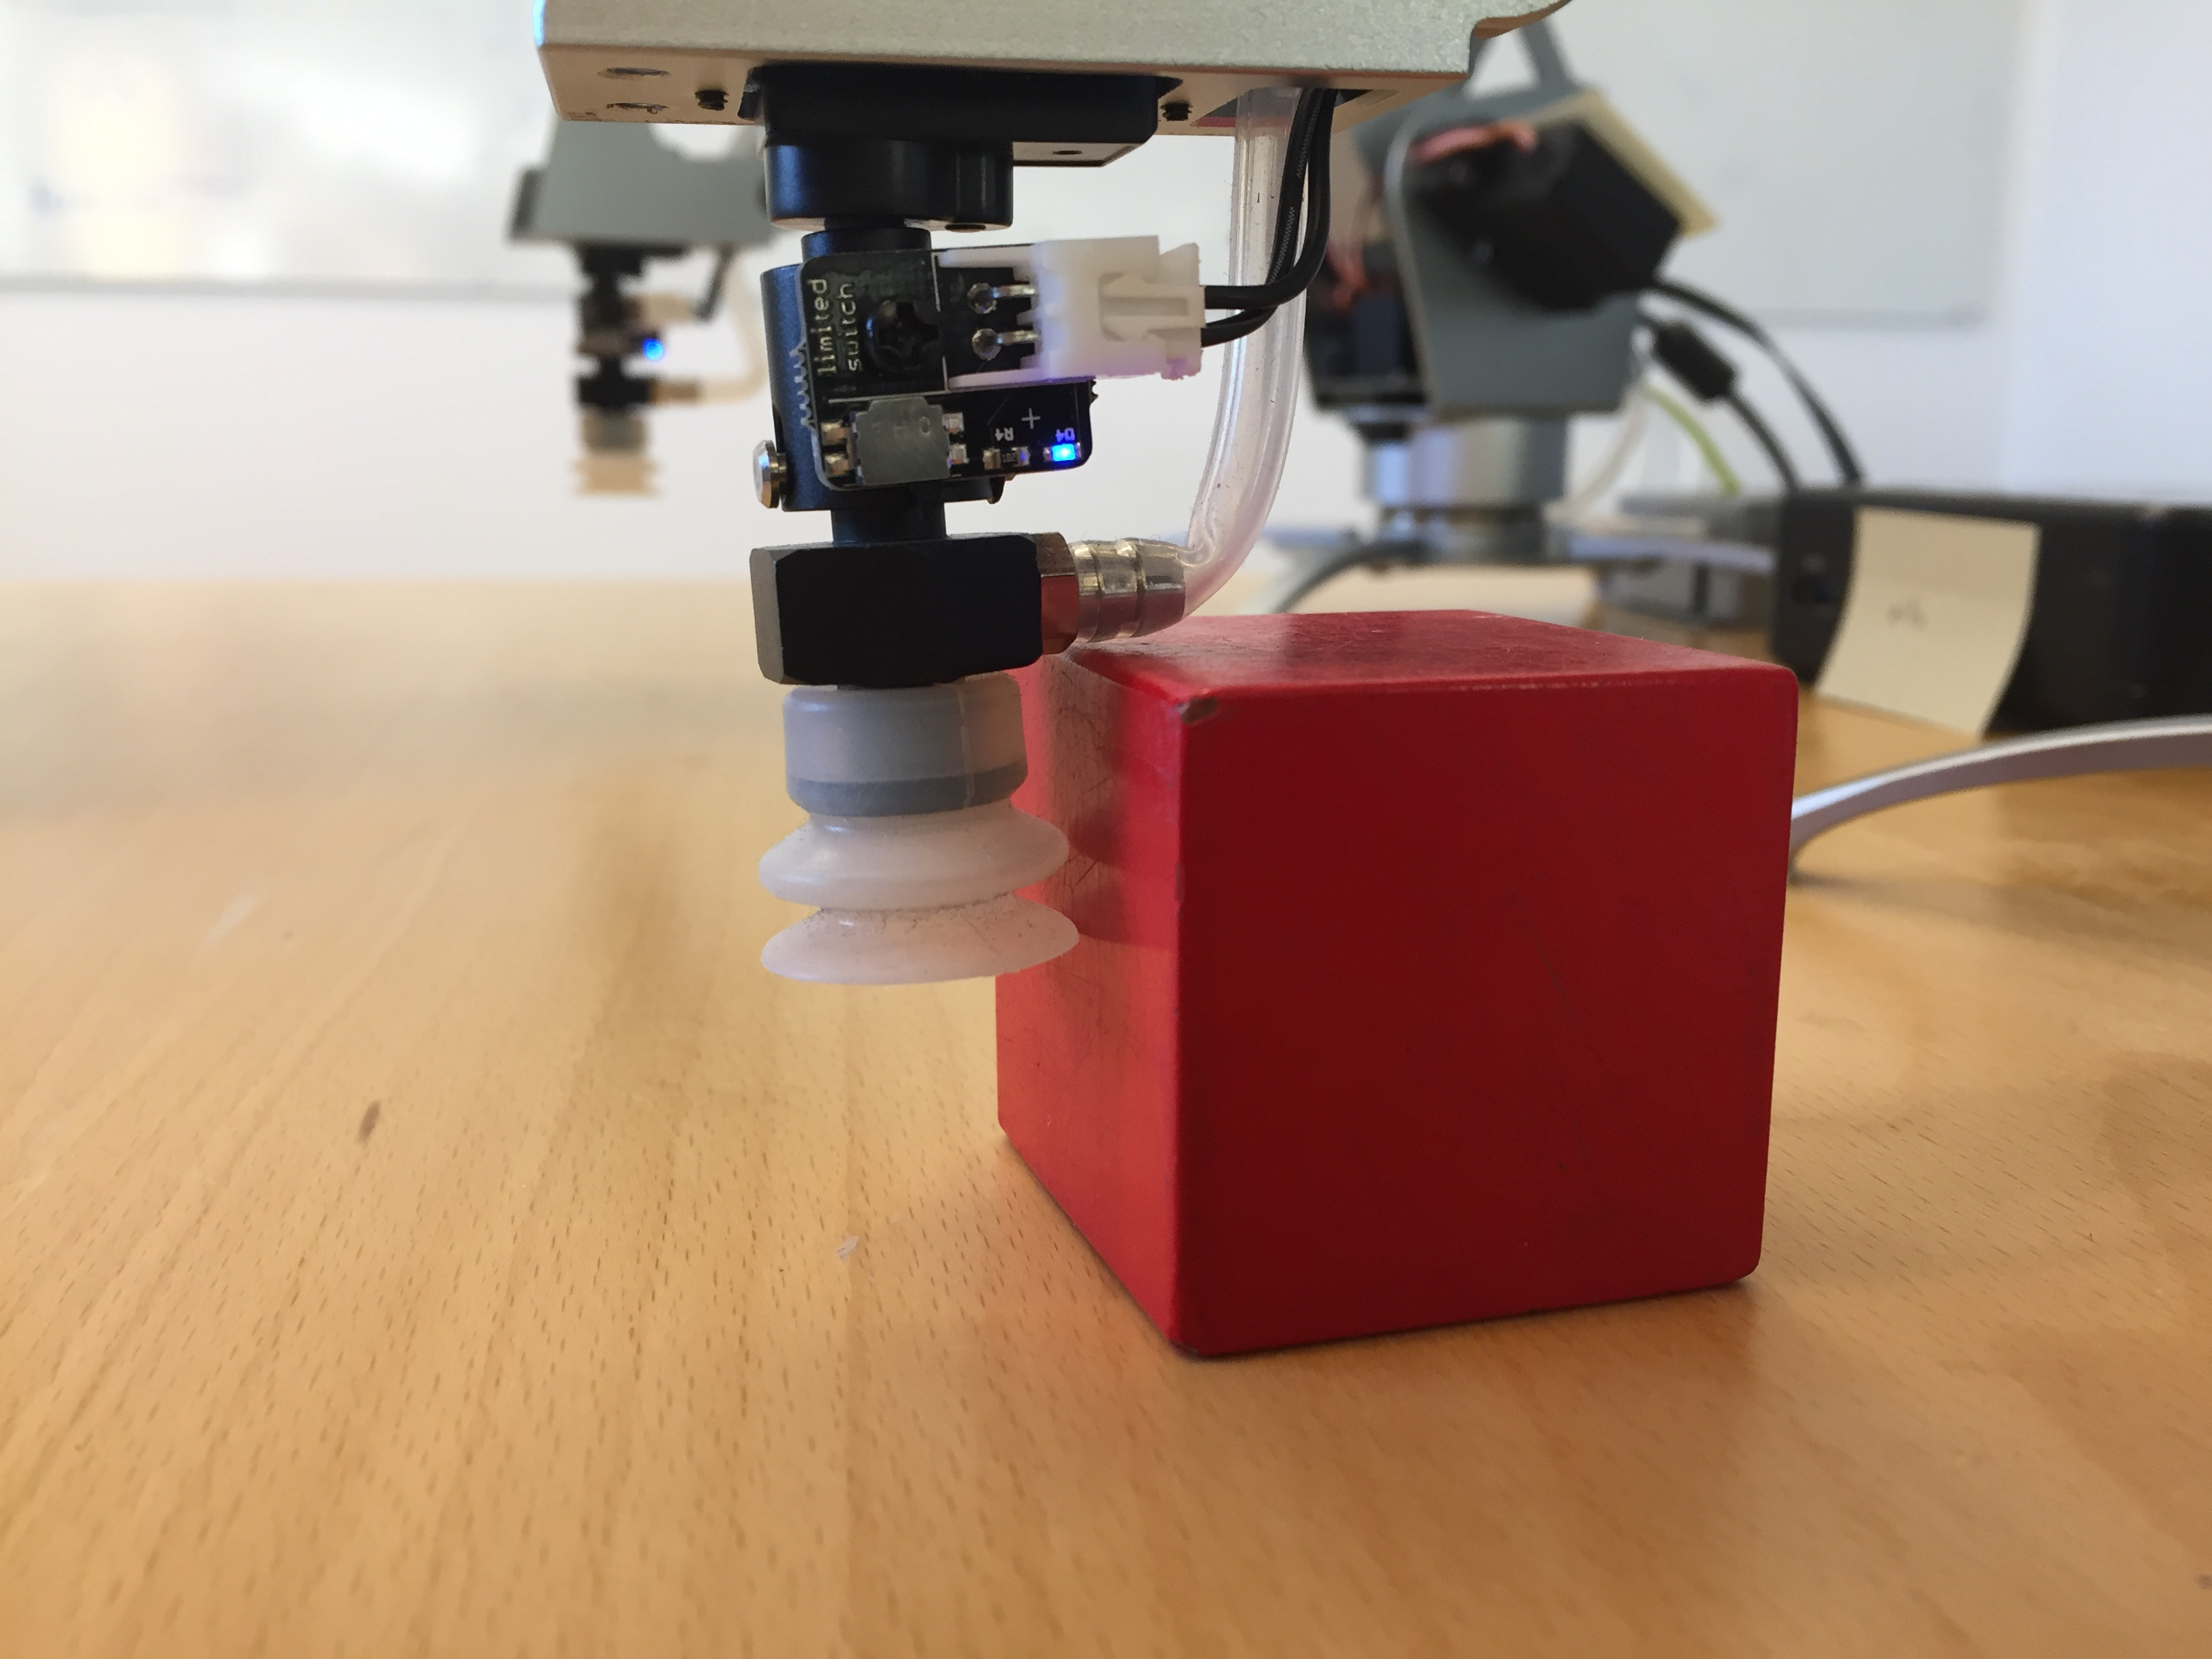
\includegraphics[width=0.40 \textwidth]{res/eef_cube_low.jpg}
%    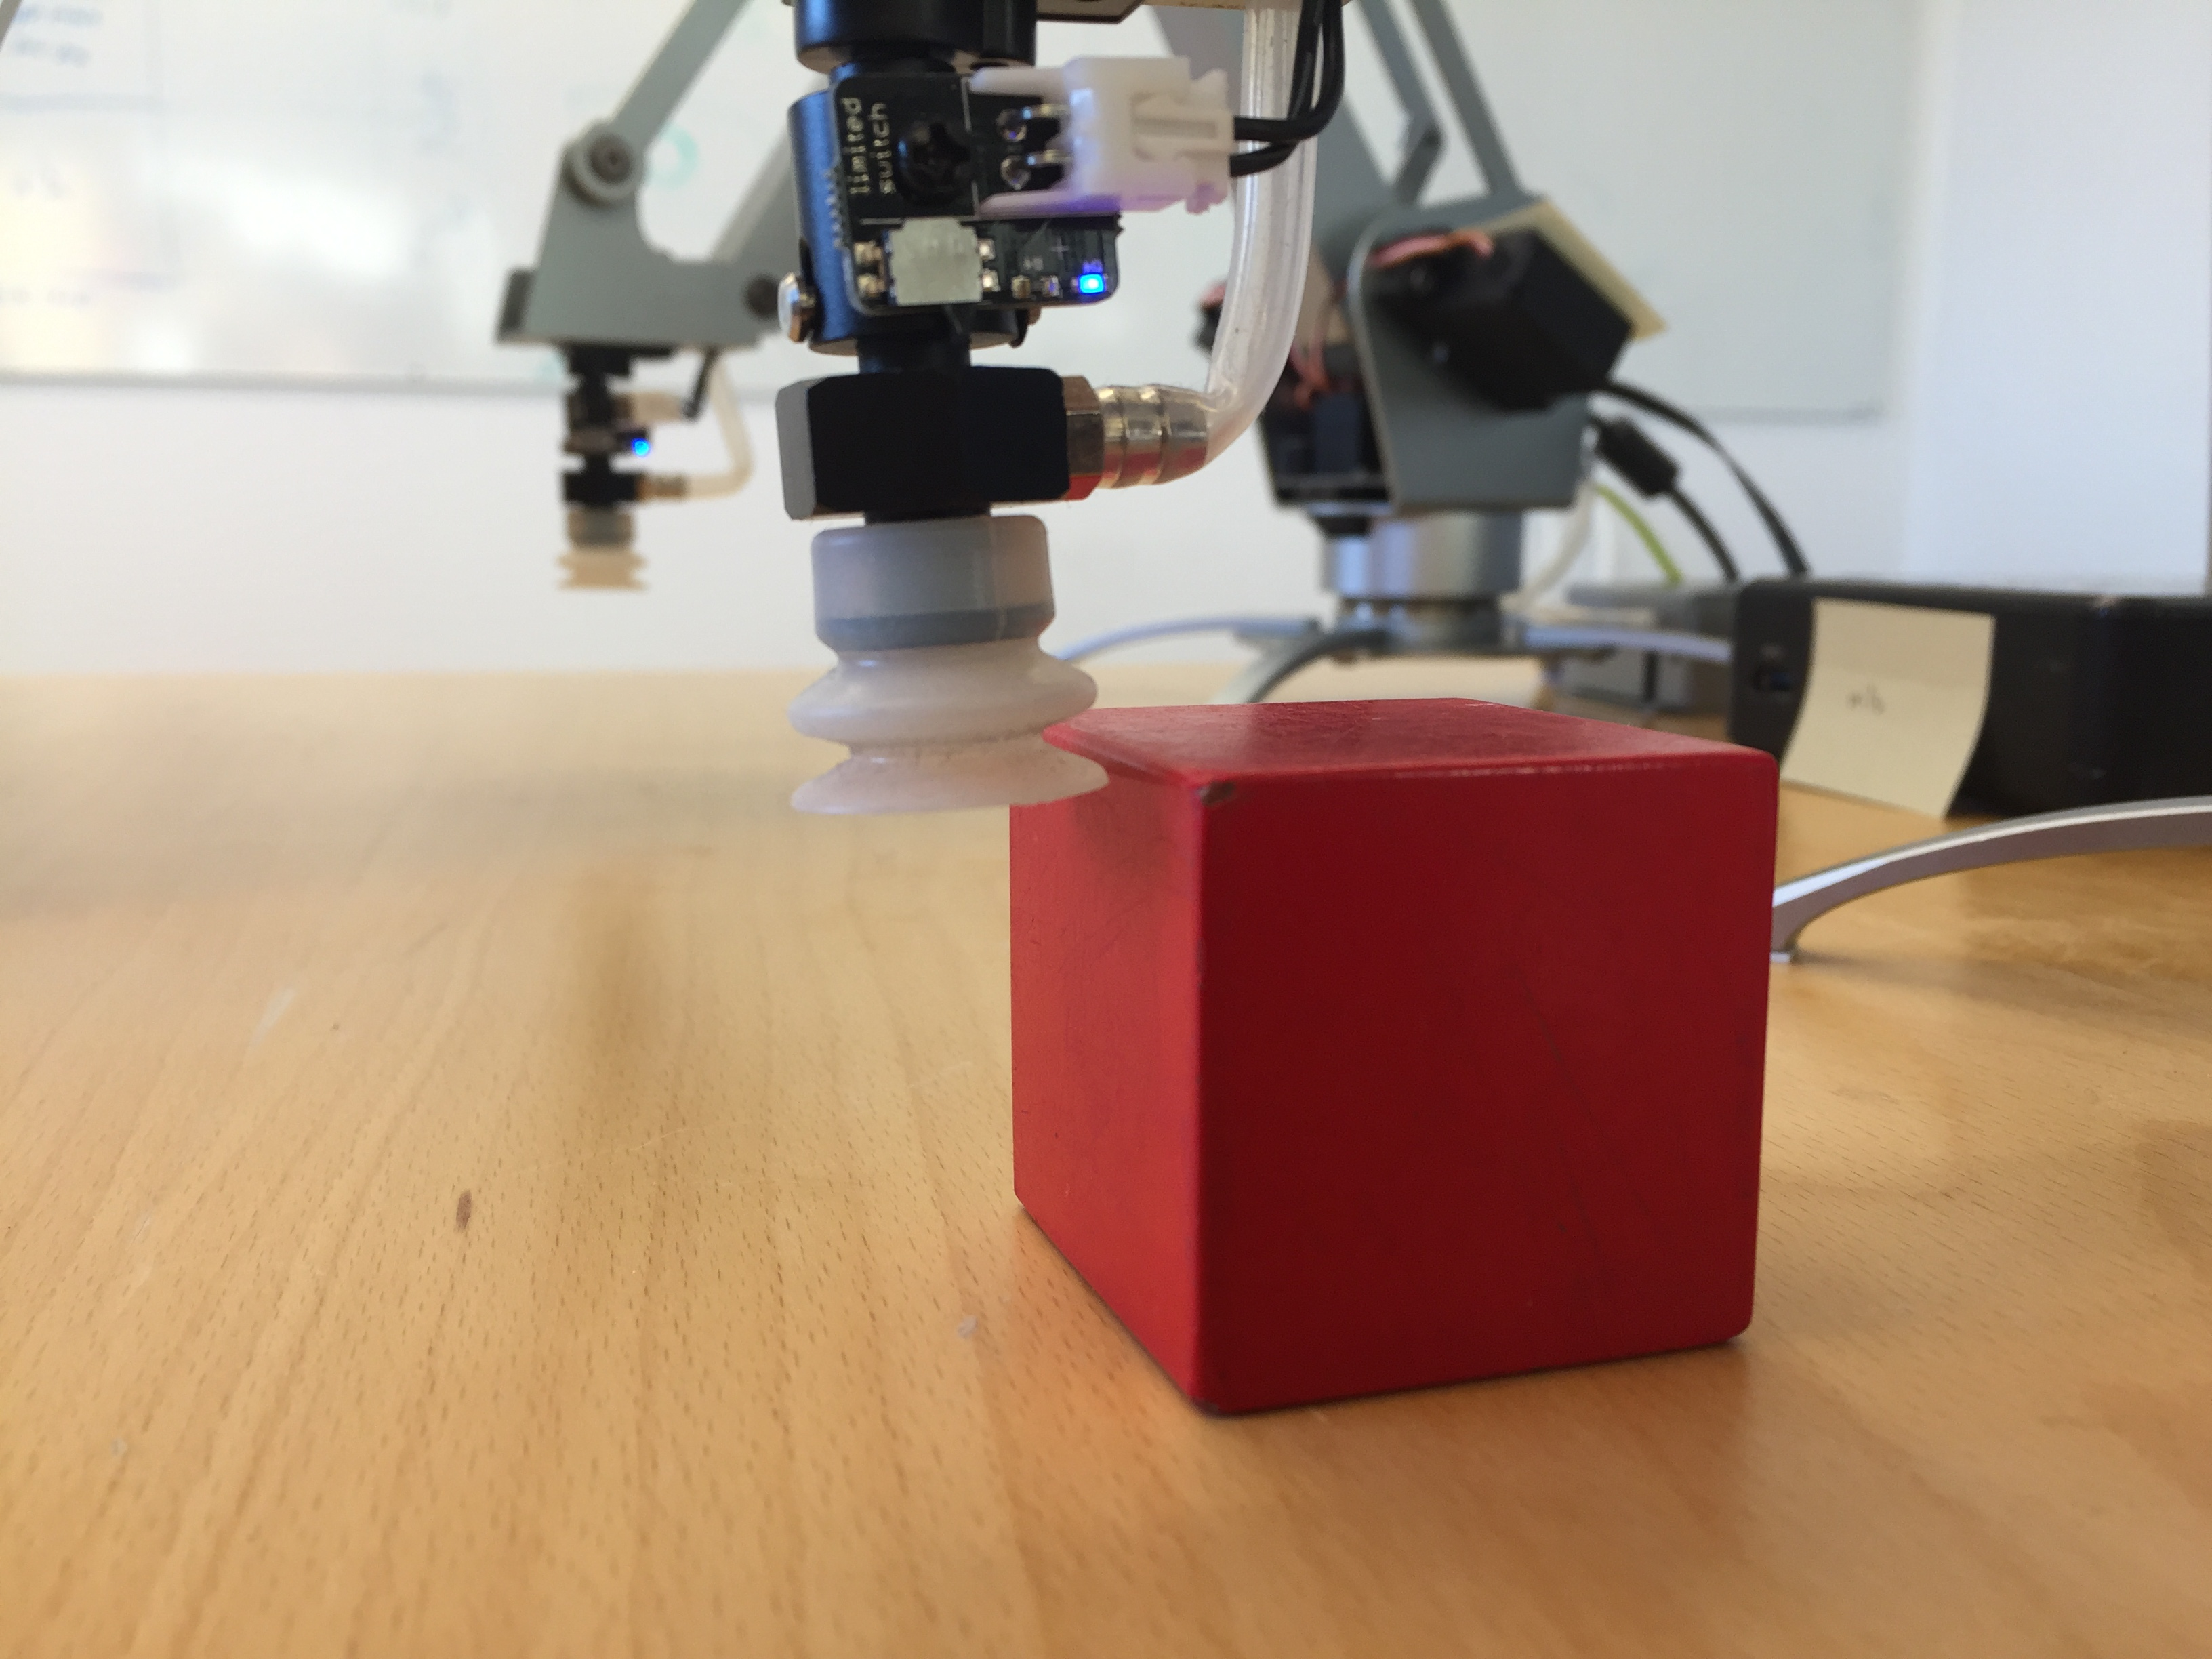
\includegraphics[width=0.40 \textwidth]{res/eef_cube_high.jpg}
%
%    \caption{Possible $z$-values of the eef. TODO: Finish/polish this}
%    
%\end{figure}
